\section{Introduction}
\only<presentation>{
  \begin{frame}
    \tableofcontents[ 
    currentsection, 
    hideothersubsections, 
    sectionstyle=show/shaded
    ] 
  \end{frame}
}

\begin{frame}
  \frametitle{Headaches and aspirins}
  \only<article>{Causal questions do not just deal with statistical relationships. The meaning of these questions is slightly different depending on whether we are talking about the population at large, or a specific individual. For populations, the main question is whether or not our actions have a causal effect. In observational data, we also need to consider the \emph{direction of causation}.}
  \begin{example}[Population effects]
    \begin{figure}[H]
      \centering
      \begin{subfigure}{\fwidth}
        \centering
        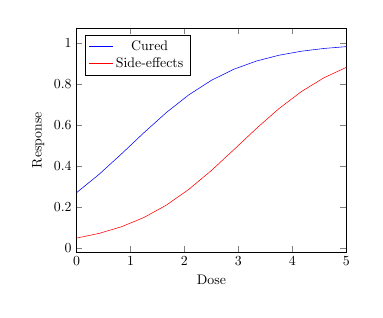
\begin{tikzpicture}[scale=0.5]
          \begin{axis}[xmin=0,xmax=5, xlabel={Dose}, ylabel={Response}, legend pos=north west]
            % use TeX as calculator:
            \addplot[color=blue] {1/(1 + e^(1-x))};
            \addplot[color=red] {1/(1 + e^(3-x))};
            \legend{Cured, Side-effects}
          \end{axis}
        \end{tikzpicture}
        \caption{Dose-response curve.}
        \label{fig:dose-response}
      \end{subfigure}
      \hspace{2em}
      \begin{subfigure}{\fwidth}
        \centering
        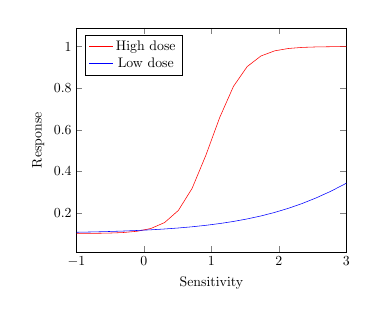
\begin{tikzpicture}[scale=0.5]
          \begin{axis}[xmin=-1,xmax=3, xlabel={Sensitivity}, ylabel={Response}, samples=50, legend pos=north west ]
            % use TeX as calculator:
            \addplot[color=red] {0.1 + 0.9*e^(4*(x-1))/(1+e^(4*(x-1)))};
            \addplot[color=blue] {0.1 + 0.9*e^(x-4)/(1+e^(x-4))};
            \legend{High dose, Low dose}
          \end{axis}
        \end{tikzpicture}
        \caption{Response sensitivity}
        \label{fig:dose-sensitivity}
      \end{subfigure}
      \caption{Investigating the response of the population to various doses of the drug.}
    \end{figure}
    \only<article>{
      We can ask ourselves two different questions about the effect of population effect aspirin on headaches.
    }
    \begin{itemize}
    \item Is aspirin an effective cure for headaches?
    \item Does having a headache lead to aspirin-taking?
    \end{itemize}
  \end{example}
  \only<article>{To examine the effect of aspirin on the population, we can look at the dose-response curve in Figure~\ref{fig:dose-response}. We first have to define what it means to be 'cured'. We also need to define possible side-effects. We can then measure how increased doses of aspirin lead to different outcomes. If the experiment has been properly conducted, this dose-response curve suggests that aspirin does have an effect in curing headaches, though it also has some side-effects. However, not all individuals are the same. Let us assume each person has a different \emph{sensitivity} to aspirin, so that some individuals responds better to treatment, especially at high doses, and some do not respond very much at all, as shown in Figure~\ref{fig:dose-sensitivity}}

\end{frame}
\begin{frame}
  \only<article>{For individuals, the first question is,  what is the possible effect of our actions? This is called the \emph{effect of causes}. The second question is, what was the reason for something happening? That is called the \emph{cause of effects?} }
  \begin{example}[Individual effects]
    \begin{figure}[H]
      \centering
      \begin{subfigure}{\fwidth}
        \includegraphics[width=\fwidth]{../figures/aspirin}
      \end{subfigure}
      \begin{subfigure}{\fwidth}
        \includegraphics[width=\fwidth]{../figures/450px-Migraine.jpg}
      \end{subfigure}
    \end{figure}
    \only<article>{
      We can ask ourselves two different questions about the individual effect of aspirin on headaches.
    }
    \begin{itemize}
    \item Effects of \alert{Causes}: Will \alert{my} headache pass \alert{if I take} an aspirin?
    \item \alert{Causes} of Effects: Would \alert{my} headache have passed if I had \alert{not taken} an aspirin?
    \end{itemize}
  \end{example}
  \only<article>{In order to be able to meaningfully talk about effects and causes we must also introduce decisions. Formally, there is nothing different in the decisions in this section and those introduced in Section~\ref{sec:decision-problems}. However, in this case we will try and use decisions to model outside interventions in a ``natural'' system, whereby a \emph{null} decision means that we do not intervene.}
\end{frame}

\begin{frame}
  \frametitle{Overview}
  \begin{block}{Inferring causal models}
    We can distinguish different \alert{models} from observational or experimental data.
  \end{block}

  \begin{block}{Inferring individual effects}
    The effect of possible intervention on an individual is not generally determinable. We usually require strong assumptions.
  \end{block}
  
  \begin{block}{Decision-theoretic view}
    There are many competing approaches to causality. We will remain within the decision-theoretic framework, which allows us to crisply define both our knowledge and assumptions.
  \end{block}
\end{frame}

\begin{frame}
  \frametitle{What causes what?}
  \begin{example}
    \begin{figure}[H]
      \centering
      \begin{subfigure}{\fwidth}
        \centering
        \begin{tikzpicture}
          \node[RV, hidden] at (0,1) (p) {$\param$};
          \node[RV] at (-1,0) (x1) {$a_t$};
          \node[RV] at (1,0) (x2) {$x_t$};
          \draw[->] (p) -- (x1);
          \draw[->] (p) -- (x2);
          \draw[->] (x1) -- (x2);
        \end{tikzpicture}
        \caption{Independence of $a_t$.}
      \end{subfigure}
      \begin{subfigure}{\fwidth}
        \centering
        \begin{tikzpicture}
          \node[RV, hidden] at (0,1) (p) {$\param$};
          \node[RV] at (-1,0) (x1) {$a_{t}$};
          \node[RV] at (1,0) (x2) {$x_{t}$};
          \draw[->] (p) -- (x1);
          \draw[->] (p) -- (x2);
          \draw[->] (x2) -- (x1);
        \end{tikzpicture}
        \caption{Independence of $x_t$.}
      \end{subfigure}
    \end{figure}
    Suppose we have data $x_{t}, a_{t}$ where
    \begin{itemize}
    \item $x_{t}$: lung cancer
    \item $a_{t}$: smoking
    \end{itemize}
    Does smoking cause lung cancer or does lung cancer make people smoke? Can we compare the two models above to determine it?
  \end{example}
  \only<article>{The answer is no. Let us consider two different parametrisations of the distribution. One in which $a_t$ generates $x_t$, and the converse, for any given parameter value $\param$, as given below:}
  \uncover<2>{
    \[
    P_\param(D) =
    \prod_t P_\param(x_t, a_t)
    = 
    \prod_t P_{\param'}(x_t \mid a_t) P_{\param'}(a_t)
    = 
    \prod_t P_{\param''}(a_t \mid x_t) P_{\param''}(x_t).
    \]
  }
  \only<article>{In particular, for any parametrisation $\param$ of the joint distribution, there exists a $\param'$ and $\param''$ giving the same probabilities for all $x_t, a_t$. For the example above, we can look at Bernoulli distributions for both variables so that $P_\param(x_t = x, a_t = a) = \param_{x,a}$. Then
    \begin{align*}
      \param'_a &= \sum_x \param_{x,a},
      &
        \param'_{x|a} &= \param_{x,a} / \param'_a
      \\
      \param''_x &= \sum_a \param_{x,a},
      &
        \param'_{a|x} &= \param_{x,a} / \param''_x.
    \end{align*}
    This means we can define prior distributions $\bel, \bel', \bel''$ in these three parameter spaces that give exactly the same results, e.g. by modelling each parameter as an independent Beta distribution. So, clearly simply looking at a simple graphical model does not let us answer this question.}
\end{frame}

\subsection{Decision diagrams}
\only<article>{
  However, graphical models \alert{can} be extended  to model causal relations. In particular, we can use \emph{decision diagrams}\footnote{Otherwise called influence diagrams}, which include not only random variables, but also \emph{decision} variables, denoted with squares, as well as utility variables, denoted via diamonds. In the following examples, we assume there are some underlying distributions specified by parameters $\param$, which we include in the diagrams for clarity. Even though it may seem intuitively sensible to suppose it, the arrow directions in the diagrams \emph{do not} indicate direct causes. The only important thing for determining whether some variable influences another is whether or not there is independence between the corresponding decision and random variables.}
\begin{frame}
  \begin{figure}[H]
    \centering
    \begin{tikzpicture}
      \node[RV, hidden] at (-1,1) (p) {$\param$};
      \node[RV] at (0,0) (x) {$x_t$};
      \node[RV] at (1,1) (y) {$y_t$};
      \only<1,2>{
        \node[select] at (2,0) (a) {$a_t$};
      }
      \only<3->{
        \node[RV] at (2,0) (a) {$a_t$};
      }
      \draw[->] (x)--(y);
      \draw[->] (x)--(a);
      \draw[->] (a)--(y);
      \draw[->] (p) to (x);
      \draw[->] (p)--(y);
      \onslide<3->{
        \node[select] at (4,0) (pol) {$\pol$};
        \draw[->] (pol)--(a);
      }
      \onslide<2->{
        \node[utility] at (3,1) (u) {$\util$};
        \draw[->] (a)--(u);
        \draw[->] (y)--(u);
      }
    \end{tikzpicture}
    \caption{A typical decision diagram where $x_t$: individual information, $y_t$: individual result, $a_t$: action, $\pol$: policy}
    \label{fig:decision-diagram}
    \index{policy!intervention}
  \end{figure}
  \only<3>{
    \begin{example}[Taking an aspirin]
      \only<article>{The diagram in Figure~\ref{fig:decision-diagram} does not completely specify the decision problem. For aspirin taking, we can define the following variables:}
      \begin{itemize}
      \item Individual $t$
      \item Individual information $x_t$
      \item $a_t  = 1$ if $t$ takes an aspirin, and $0$ otherwise.
      \item $y_t = 1$ if the headache is cured in 30 minutes, $0$ otherwise.
      \item $\pol$: intervention policy.\index{policy!intervention}
      \end{itemize}
    \end{example}
  }
  \only<4>{
    \begin{example}[A recommendation system]
      \only<article>{Consider the example of a recommendation system, where we have data of the form $(x_t, a_t, y_t)$. The performance of the recommendation system depends not only on the parameter $\param$, but also on the chosen policy $\pol$. }
      \begin{itemize}
      \item $x_t$: User information (random variable)
      \item $a_t$: System action (random variable)
      \item $y_t$: Click (random varaible)
      \item $\pol$: recommendation policy (decision variable).\index{policy!recommendation}
      \end{itemize}
    \end{example}
  }
  \only<article>{In both cases, there are some questions we can ask using the underlying model. The dependency structure is not enough to know \emph{a priori} whether we can obtain meaningful answers. This depends on the specific assumptions we make about the model.}
\end{frame}

\begin{frame}
  \frametitle{Conditional distributions and decision variables.}
  \only<article>{We begin with a parenthesis on conditional distributions. We normally define the conditional distribution of $A$ given $B$ under a probability measure $P$ as:}
  \[
  P(A \mid B) \defn \frac{P(A \cap B)}{P(B)}.
  \]
  \only<article>{However, decision variables are outside the scope of this probability measure, and yet we need to define conditional distributions using them. }
  \begin{block}{The conditional distribution of decisions}
    \only<article>{If $\pol \in \Pol$ is a decision variable, we represent the conditional distribution of any random variable $a$ given $\pol$ simply as a collection of probability measures $\cset{\pol(a)}{\pol \in \Pol}$, one for each possible value $\pol$. The following notations will be equivalent:}
    \[
    \pol(a) \equiv \Pr^\pol(a) \equiv \Pr(a \mid \pol).
    \]
    \only<article>{The reader should note that the standard definition of a conditional distribution also $P(A \mid B)$ creates a collection of distributions on $A$, with elements $P_B(A)$. However, it also specifies a rule for doing so from the complete distribution $P$. 

      If the random variables $a$ also depends on some probability law $P_\param$, then it will be convenient to use the notation
    }
    \[
    \Pr_\param^\pol(a) \equiv \Pr(a \mid \param, \pol).
    \]
  \end{block}
\end{frame}
\subsection{Common structural assumptions}
\only<article>{
  In order to be clear about what constitutes an observation by the experimenter and what is a decision, we must clearly separate random variables from decision variables. The individual actions may be random variables, but they will depend on decisions taken. As we will see later, this is useful for modelling interventions.}

\begin{frame}
  \frametitle{Basic causal structures}
  \only<article>{Directed graphical models are not sufficient to determine causality by themselves, as they only determine correlations between random variables. If we have decision variables, however, we can always determine whether or not our decisions influence outcomes.}
  \begin{block}{Non-cause}
    \begin{figure}[H]
      \centering
      \begin{tikzpicture}
        \node[select] at (0,0) (p) {$\pol$};
        \node[RV] at (1,0) (a) {$a_t$};
        \node[RV] at (2,0) (y) {$y_t$};
        \draw[->] (p) to (a);
        \draw[->] (y) to (a);
        \uncover<2>{
          \node[RV, hidden] at (1,1) (param) {$\param$};
          \draw[->] (param) to (y);
        }
      \end{tikzpicture}
      \caption{$\pol$ does not cause $y$}
      \label{fig:non-cause}
    \end{figure}
    \only<article>{In the diagram above, we see that $y_t \indep \pol$.}
  \end{block}
  \only<article>{
    \begin{example}
      Consider the model
      \begin{align*}
        y_t &\sim \Normal(0,1)\\
        a_t \mid y_t, \pol &\sim \Normal(y_t + \pol, 1)
      \end{align*}
      \begin{figure}[H]
        \centering
        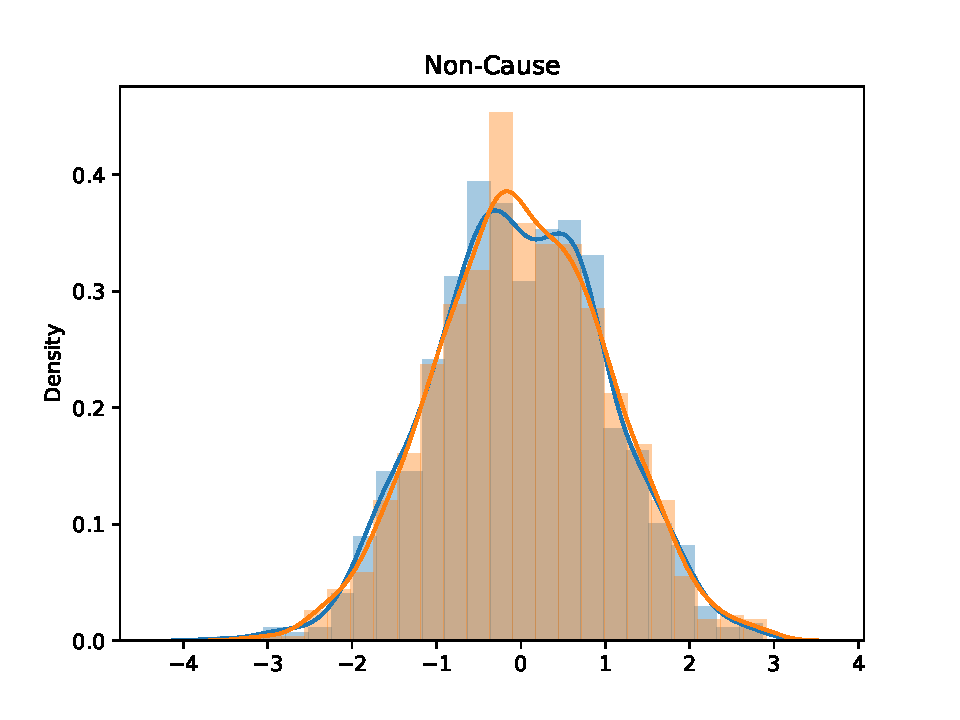
\includegraphics[width=0.5\textwidth]{../src/causality/non-cause}
        \caption{$\Pr^\pol(y_t)$ for $\pol \in \{-1, 1\}$ when $\pol$ is not a cause for $y_t$}
        \label{fig:non-cause-dist}
      \end{figure}
      In this example, we see tht $y_t$ is independent of the policy
      $\pol$.  However, $y_t$ is not independent of the action taken, as the action depends on $y_t$ directly. The correlation between $y, a$ is shown in Figure~\ref{fig:a-y-correlation:non-cause}.
    \end{example}
  }
  
  \begin{block}{No confounding}
    \only<article>{Confounding is a term that indicates the existence of latent variables that create dependencies between $y_t, \pol, a_t$. We are sure that there is no confounding whenever $y_t \indep \pol \mid a_t$, as captured by the diagram in Figure~\ref{fig:no-confounding}. In this case $\pol$ is a direct cause for $y_t$ through $a_t$.}
    \begin{figure}[H]
      \centering
      \begin{tikzpicture}
        \node[select] at (0,0) (p) {$\pol$};
        \node[RV] at (1,0) (a) {$a_t$};
        \node[RV] at (2,0) (y) {$y_t$};
        \draw[->] (p) to (a);
        \draw[->] (a) to (y);
        \uncover<2>{
          \node[RV, hidden] at (1,1) (param) {$\param$};
          \draw[->] (param) to (y);
        }
      \end{tikzpicture}
      \caption{No confounding: $\pol$ causes $y_t$}
      \label{fig:no-confounding}
    \end{figure}
  \end{block}

  \only<article>{
    \begin{example}
      Consider the model
      \begin{align*}
        a_t &\sim \Normal(\pol,1)\\
        y_t \mid a_t, \pol &\sim \Normal(a_t, 1)
      \end{align*}
      \begin{figure}[H]
        \centering
        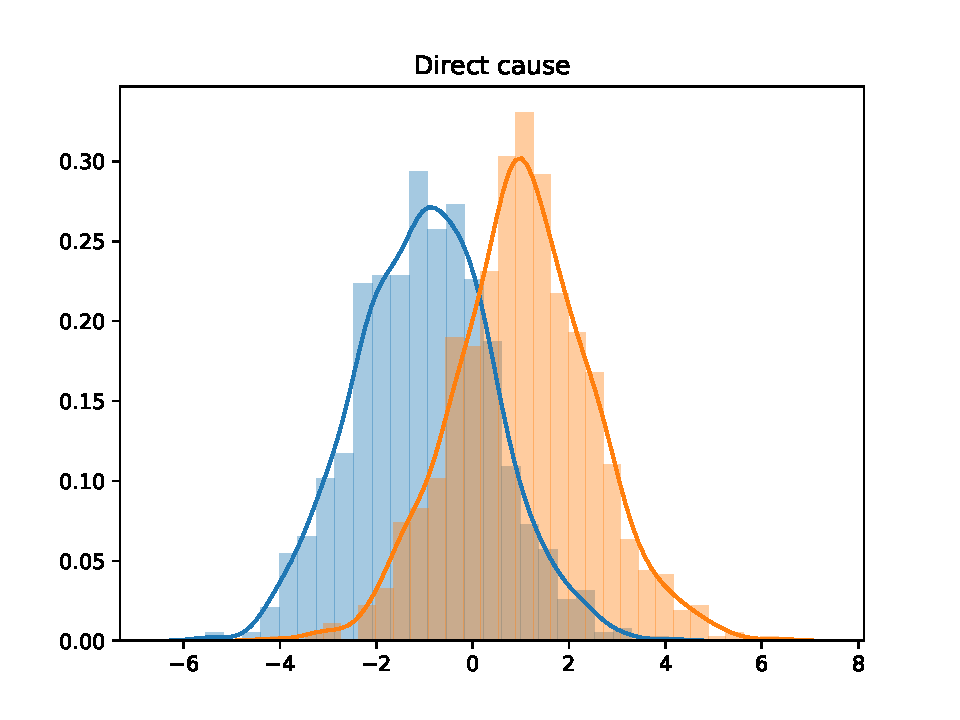
\includegraphics[width=0.5\textwidth]{../src/causality/direct-cause}
        \caption{$\Pr^\pol(y_t)$ for $\pol \in \{-1, 1\}$ when $\pol$ is a direct cause for $y_t$}
        \label{fig:non-cause-dist}
      \end{figure}
      \only<article>{We can see how the distribution of $y_t$ changes when $\pol$ changes in Figure~\ref{fig:non-cause-dist}. In this case there is also a correlation between $a_t, y_t$ as seen in Figure~\ref{fig:a-y-correlation}.}
    \end{example}
  }

  \only<article>{
    \begin{figure}[H]
      \centering
      \begin{subfigure}{0.45\textwidth}
        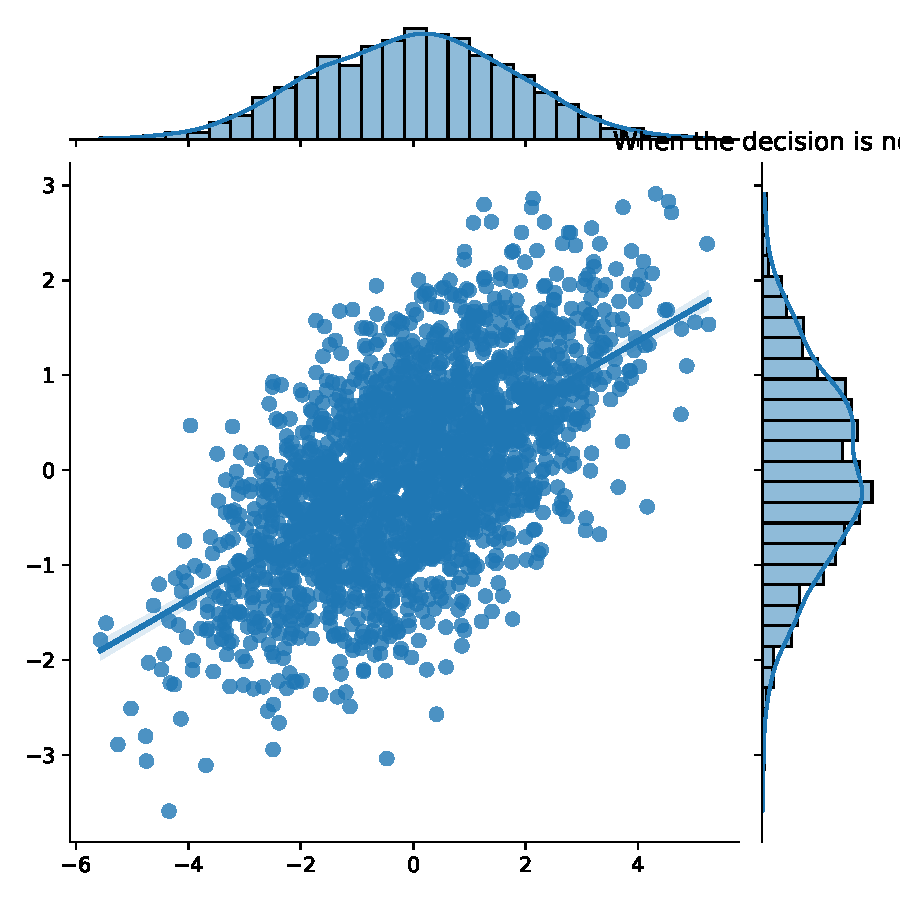
\includegraphics[width=0.9\textwidth]{../src/causality/a-y-non-cause}
        \caption{Non-cause}
        \label{fig:a-y-correlation:non-cause}
      \end{subfigure}
      \hspace{1em}
      \begin{subfigure}{0.45\textwidth}
        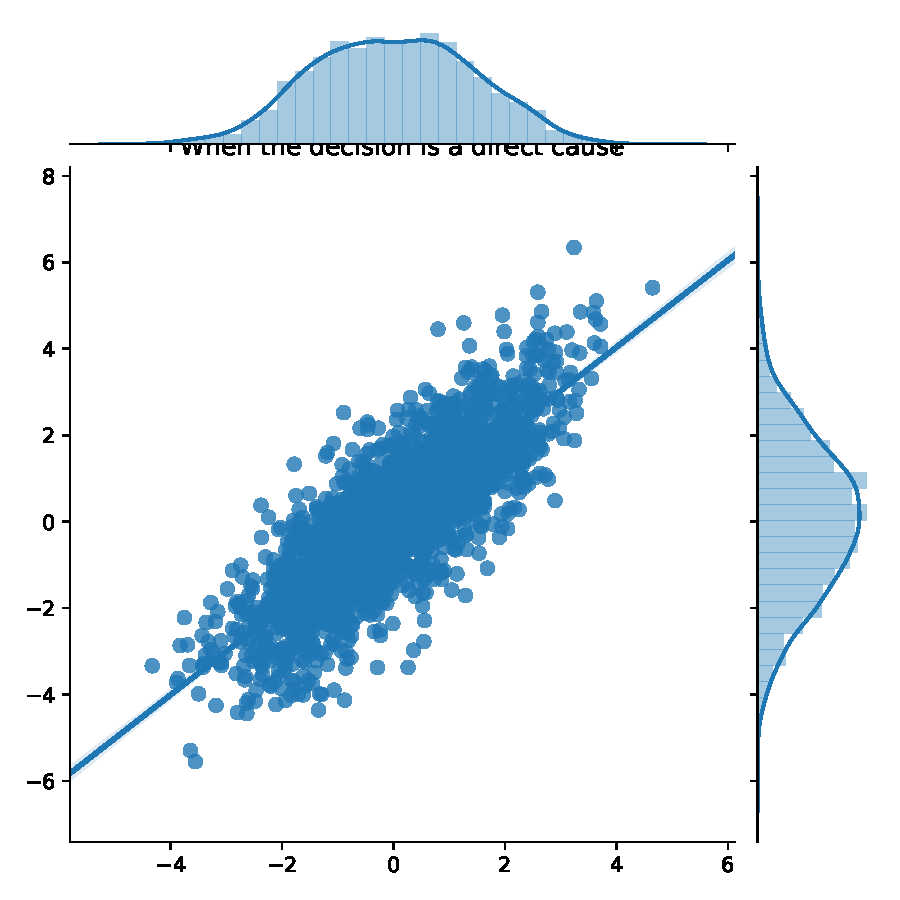
\includegraphics[width=0.9\textwidth]{../src/causality/a-y-direct-cause}
        \caption{Cause}
        \label{fig:a-y-correlation:cause}
      \end{subfigure}
      \caption{Correlation between $a_t$ and $y_t$}
      \label{fig:a-y-correlation}
    \end{figure}
  }
\end{frame}
\begin{frame}
  \frametitle{Covariates}
  \begin{block}{Sufficient covariate}
    \only<article>{Sometimes the variable of interest is not conditionally independent of the treatment, unless there exists a \emph{sufficient covariate} $x_t$ such that
      $y_t \indep \pol \mid a_t, x_t$. If $x_t$ is not observed, then it is sometimes called a confounder.}
    \begin{figure}[H]
      \centering
      \begin{tikzpicture}
        \node[select] at (0,0) (p) {$\pol$};
        \node[RV] at (1,0) (a) {$a_t$};
        \node[RV] at (2,0) (y) {$y_t$};
        \node[RV] at (2,1) (x) {$x_t$};
        \draw[->] (p) to (a);
        \draw[->] (a) to (y);
        \draw[->] (x) to (a);
        \draw[->] (x) to (y);
        \uncover<2>{
          \node[RV, hidden] at (3,1) (param) {$\param$};
          \draw[->] (param) to (x);
          \draw[->] (param) to (y);
        }
      \end{tikzpicture}
      \caption{Sufficient covariate $x_t$}
      \label{fig:sufficient-covariate}
    \end{figure}
  \end{block}

  \only<article>{
    \begin{example}
      Consider the model
      \begin{align*}
        x_t &\sim \Normal(0, 1)\\
        a_t &\sim \Normal(x_t + \pol, 1)\\
        y_t \mid a_t, \pol &\sim \Normal(x_t + a_t, 1),
      \end{align*}
      \only<article>{Here $x_t$ influences the outcome $y_t$, but also directly influences $a_t$ through the policy $\pol$. As we can see in Figure~\ref{fig:non-cause-dist}, the policy then has an influence on $y_t$}
      \begin{figure}[H]
        \centering
        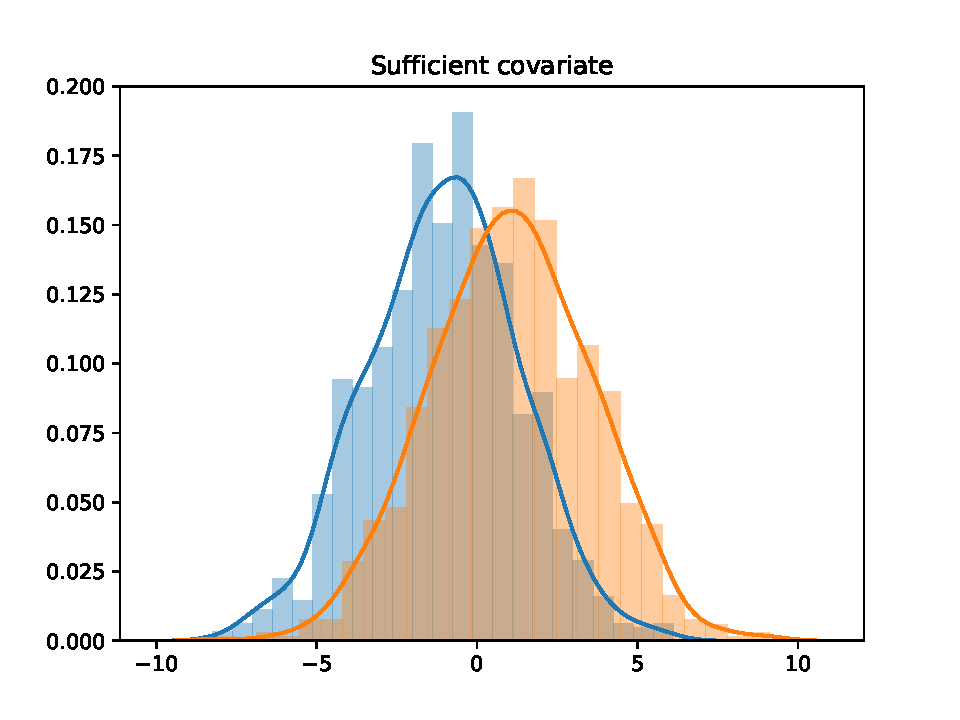
\includegraphics[width=0.5\textwidth]{../src/causality/sufficient}
        \caption{$\Pr^\pol(y_t)$ for $\pol \in \{-1, 1\}$ when $\pol$ is a direct cause for $y_t$}
        \label{fig:sufficient-covariate-dist}
      \end{figure}
    \end{example}
  }


  \begin{block}{Instrumental variables and confounders}
    \only<article>{If the sufficient covariate $x_t$ is not observed, we may still have another variable available, $z_t$, on the basis of which we make our decisions. This is called an \emph{instrumental variable.} \index{instrument@see{variable!instrumental}}\index{variable!instrumental}. In this case $z_t$ still depends on $x_t$ and the effect of the treatment depends on $x_t$ directly. As $x_t$ is a latent covariate, it can be called a \emph{confounder.} \index{confounder}}
    \begin{figure}[H]
      \centering
      \begin{tikzpicture}
        \node[select] at (0,0) (p) {$\pol$};
        \node[RV] at (1,0) (a) {$a_t$};
        \node[RV] at (2,0) (y) {$y_t$};
        \node[RV, hidden] at (2,1) (x) {$x_t$};
        \node[RV] at (1,1) (z) {$z_t$};
        \draw[->] (p) to (a);
        \draw[->] (a) to (y);
        \draw[->] (x) to (y);
        \draw[->] (x) to (z);
        \draw[->] (z) to (a);
        \uncover<2>{
          \node[RV, hidden] at (3,1) (param) {$\param$};
          \draw[->] (param) to (x);
          \draw[->] (param) to (y);
          \draw[bend right=45,->] (param) to (z);
        }
      \end{tikzpicture}
      \caption{Instrumental variable $z_t$}
      \label{fig:instrumental-variable}
    \end{figure}
  \end{block}

  \only<article>{
    \begin{example}
      Consider the model
      \begin{align*}
        x_t &\sim \Normal(0, 1)\\
        z_t &\sim \Normal(x_t, 1)\\
        a_t &\sim \Normal(z_t + \pol, 1)\\
        y_t \mid a_t, \pol &\sim \Normal(x_t + a_t, 1)
      \end{align*}
      \only<article>{In this scenario, $x_t$ directly influences the outcome $y_t$, but is not observed.\footnote{Hence, it can be called a confounder.}}
      \begin{figure}[H]
        \centering
        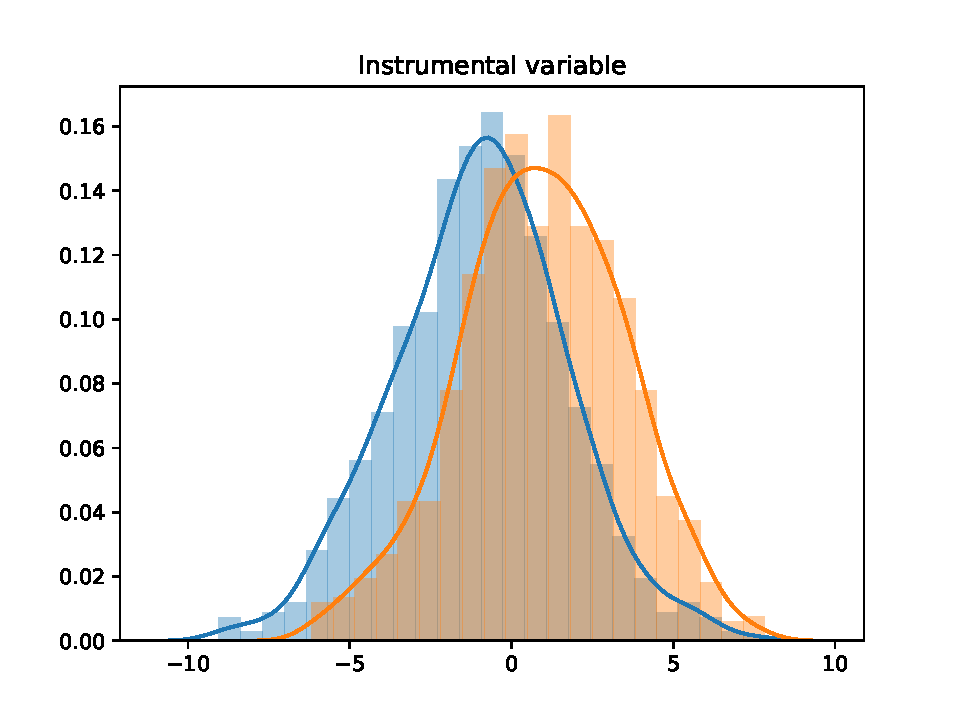
\includegraphics[width=0.5\textwidth]{../src/causality/instrumental}
        \caption{$\Pr^\pol(y_t)$ for $\pol \in \{-1, 1\}$ when $\pol$ is a direct cause for $y_t$}
        \label{fig:instrumental-dist}
      \end{figure}
    \end{example}
  }


\end{frame}


\section{Interventions}
\only<article>{Interventions are of primary interest when we have a set of observational data, collected under a \emph{null} or \emph{default} policy $\pol_0$.  We then wish to intervene with some policy $\pol$ in order to maximise our utility function, or to simply try and estimate the exact relationships between variables.}
\begin{frame}
  \frametitle{Modelling interventions}
  \begin{itemize}
  \item Observational data $D$. \only<article>{This represents data we have collected from some previous regime. In order to be able to model the problem precisely, we must posit the existence of some default policy $\pol_0$ under which the data was collected.}
  \item Policy space $\Pol$. \only<article>{This must include $\pol_0$, as well as any other policies that the decision maker may be able to choose in the future.} 
  \end{itemize}
  \begin{block}{Default policy}
    \index{policy!default}
    The space of policies $\Pol$ includes a \alert{default policy} $\pol_0$, under which the data was collected. \only<article>{The policy $\pol_0$ might already be known, if for example the data was collected with a specific algorithm. However, frequently $\pol_0$ is not given, and must also be inferred from the data. In that case, it can be seen as an additional parameter, complementary to $\param$.}
  \end{block}
  \begin{block}{Intervention policies}
    \index{policy!intervention}
    Except $\pol_0$, policies $\pol \in \Pol$ represent different interventions specifying a distribution $\pol(a_t \mid x_t)$.
    \begin{itemize}
    \item Direct interventions. \only<article>{The simplest scenario is when we are able to choose a $\pol$ for which we know $\pol(a_t \mid x_t)$. This counts as a direct intervention, as we can specify any distribution of actions allowed in $\Pol$. If $\Pol$ includes all conditional distributions, we can select an arbitrary action for every individual. This assumption is plausible for algorithmic decision making such as recommendation systems, but implausible when the actions are taken by another agent, such as a human.}
    \item Indirect interventions and non-compliance. \only<article>{In this scenario we assume that, while we are free to choose policies from $\Pol$, we do not know what distribution $\pol(a_t \mid x_t)$ each policy specifies. In algorithmic decision making, this occurs whenever $\pol$ represents hyperparameters and algorithms for which we have insufficient information. Then policies must be evaluated through some type of black-box (e.g. A/B) testing. When the actions are taken by (human) agents, the policy implies making a recommendation, which may not be followed by the agent. If we denote the recommendation by $v_t$, then we can write $\pol(a_t \mid x_t) = \sum_{z_t} \pol(a_t \mid z_t, x_t) \pol(z_t \mid x_t)$. In this scenario we can freely specify $\pol(z_t \mid x_t)$, but $\pol(a_t \mid z_t, x_t)$ must be estimated. For that reason, it is usually simpler to simply marginalise out $a_t$. But perhaps the simplest approach is to consider non-compliance as a confounder $x_t$, and $z_t$ as an instrumental variable. }
    \end{itemize}
  \end{block}
\end{frame}
\begin{frame}
  \begin{example}[Weight loss]
    \only<article>{Consider weight loss. We can collect observational data from a population of overweight adults over a year. We can imagine that $x$ represents the weight and vital statistics of an individual and $y$ their change in weight after a year. We may also observe their individual actions $a$, such as whether or not they are following a particular diet or exercise regime. Under the default policy $\pol_0$, their actions are determined only the individuals. Consider an alternative policy $\pol$, which prescribes diet and exercise regimes. Due to non-compliance, actual actions taken by individuals may differ from prescribed actions. In addition, actions might not be observed.}
    \only<presentation>{
      \only<1>{
        \begin{figure}[H]
          \centering
                \begin{tikzpicture}
        \node[RV, hidden] at (0,1) (p) {$\param$};
        \node[RV] at (0,0) (x) {$x_t$};
        \node[RV] at (1,1) (y) {$y_t$};
        \node[RV] at (2,0) (a) {$a_t$};
        \draw[->] (p)--(x);
        \draw[->] (p)--(y);
        \draw[->] (x)--(y);
        \draw[->] (x)--(a);
        \draw[->] (a)--(y);
        \node[select] at (4,0) (p) {$\pol$};
        \draw[->] (p)--(a);
        \node[utility] at (3,1) (u) {$\util$};
        \draw[->] (a)--(u);
        \draw[->] (y)--(u);
      \end{tikzpicture}

%%% Local Variables:
%%% mode: latex
%%% TeX-master: "notes"
%%% End:

        \end{figure}
      }
    }
    \only<2>{
      \begin{figure}[H]
        \centering
        \begin{tikzpicture}
          \node[RV, hidden] at (0,1) (p) {$\param$};
          \node[RV] at (0,0) (z) {$z_t$};
          \node[RV, hidden] at (1,2) (x) {$x_t$};
          \node[RV] at (1,1) (y) {$y_t$};
          \node[RV] at (2,0) (a) {$a_t$};
          \draw[->] (p)--(z);
          \draw[->] (p)--(x);
          \draw[->] (p)--(y);
          \draw[->] (x)--(y);
          \draw[->] (z)--(y);
          \draw[->] (z)--(a);
          \draw[->] (a)--(y);
          \node[select] at (4,0) (p) {$\pol$};
          \draw[->] (p)--(a);
          \node[utility] at (3,1) (u) {$\util$};
          \draw[->] (a)--(u);
          \draw[->] (y)--(u);
        \end{tikzpicture}
        \caption{Model of non-compliance as a confounder.}
        \label{fig:non-compliance}
      \end{figure}
    }
  \end{example}
\end{frame}  


\section{Policy evaluation and optimisation}
\index{policy!evaluation}
\begin{frame}
  \frametitle{The value of an observed policy}
  \only<presentation>{
    \begin{figure}[H]
      \centering
            \begin{tikzpicture}
        \node[RV, hidden] at (0,1) (p) {$\param$};
        \node[RV] at (0,0) (x) {$x_t$};
        \node[RV] at (1,1) (y) {$y_t$};
        \node[RV] at (2,0) (a) {$a_t$};
        \draw[->] (p)--(x);
        \draw[->] (p)--(y);
        \draw[->] (x)--(y);
        \draw[->] (x)--(a);
        \draw[->] (a)--(y);
        \node[select] at (4,0) (p) {$\pol$};
        \draw[->] (p)--(a);
        \node[utility] at (3,1) (u) {$\util$};
        \draw[->] (a)--(u);
        \draw[->] (y)--(u);
      \end{tikzpicture}

%%% Local Variables:
%%% mode: latex
%%% TeX-master: "notes"
%%% End:

      \caption{Basic decision diagram}
    \end{figure}
  }
  \only<article>{
    In this section, we will focus on the general model of Figure~\ref{fig:decision-diagram}.
    If we have data $D = \cset{(x_t, a_t, y_t)}{t \in [T]}$ generated from some policy $\pol_0$, we can always infer the average quality of each action $a$ under that policy.}
  \only<2>{
    \begin{align}
      \label{eq:observed-expected-utility}
      \hat{\E}_D(U \mid a) 
      &\defn
        \frac{1}{|\cset{t}{a_t = a}|}
        \sum_{t: a_t = a}
        U(a_t, y_t)\\
      &\approx
        \E^{\pol_0}_\param (U \mid a)
      & (a_t, y_t) & \sim \Pr_\param^{\pol_0}.
    \end{align}
  }
  \only<article>{
    Can we calculate the value of another policy? As we have seen from Simpson's paradox\index{Simpson's paradox}, it is folly to simply select
  }
  \[
  \hat{a}^*_D \in \argmax_a \hat{\E}_D(U \mid a),
  \]
  \only<article>{
    as the action also depends on the observations $x$ through the policy.
    To clarify this, let us look again at the model shown in Figure~\ref{fig:decision-diagram}.
  }
\end{frame}
\begin{frame}

  \begin{align*}
    x_t \mid \param &\sim P_\param(x)\\
    y_t \mid \param, x_t, a_t &\sim P_\param(y \mid x_t, a_t)\\
    a_t \mid x_t, \pol &\sim \pol(a \mid x_t).
  \end{align*}
  \only<article>{
    Assume that $x \in \CX$, a continuous space, but $y \in \CY$ is discrete. In this scenario, then the value of an action under a policy $\pol$ is nonsensical, as it does not really depend on the policy itself:
    \begin{align*}
      \E^\pol_\param(\util \mid a)
      &=
        \int_\CX \dd P_\param(x)
        \sum_{y \in \CY} P_\param(y \mid x, a) \util(a, y).
    \end{align*}
    We see that there is a clear dependence on the distribution of $x$, and there is no dependence on the policy any more. In fact, equation above only tells us the expected utility we'd get if we always chose the same action $a$. But what is the optimal policy? First, we have to define the value of a policy.}
  \begin{block}{The value of a policy}
    \begin{align*}
      \E^\pol_\param(\util)
      &=
        \int_\CX \dd P_\param(x)
        \sum_{a \in \CA}  \pol(a \mid x)  \sum_{y \in \CY} P_\param(y \mid x, a) \util(a, y)
    \end{align*}
  \end{block}
  The optimal policy under a known parameter $\param$ is given simply by
  \begin{align*}
    \max_{\pol \in \Pol} \E^\pol_\param(\util),
  \end{align*}
  where $\Pol$ is the set of allowed policies. 
\end{frame}

\begin{frame}
  \frametitle{Monte-Carlo estimation}
  \only<article>{The simplest method to estimate the value of an alternative policy is to use Monte-Carlo estimation and importance sampling. However, this estimate can have a very high variance if the alternative policy is very different from the original policy.}
  \begin{block}{Importance sampling\footnote{Also known as Propensity Scoring}}
    We can obtain an unbiased estimate of the utility in a model-free manner through importance sampling:
    \only<presentation>{
      \begin{align*}
        \E^\pol_\param(\util)
        &=
          \int_\CX \dd P_\param(x)
          \sum_a
          \E_\param(\util \mid a, x)
          \pol(a \mid x)\\
        &\approx
          \frac{1}{T}
          \sum_{t=1}^T
          \util_t 
          \frac{\pol(a_t \mid x_t)}{\pol_0(a_t \mid x_t)}.
      \end{align*}
    }

    \only<article>{
      \begin{align*}
        \E^\pol_\param(\util)
        &=
          \int_\CX \dd P_\param(x)
          \sum_a
          \E_\param(\util \mid a, x)
          \pol(a \mid x)\\
        &\approx
          \frac{1}{T}
          \sum_a \sum_t
          \E_\param(\util \mid a, x_t)
          \pol(a \mid x_t), & x_t & \sim P_\param(x)\\
        &=
          \frac{1}{T}
          \sum_t \sum_a
          \E_\param(\util \mid a, x_t)
          \frac{\pol(a \mid x_t)}{\pol_0(a \mid x_t)} \pol_0(a \mid x_t)\\
        &\approx
          \frac{1}{T}
          \sum_{t=1}^T
          \util_t 
          \frac{\pol(a_t \mid x_t)}{\pol_0(a_t \mid x_t)},
        & a_t \mid x_t \sim & \pol_0, \quad U_t \mid x_t, a_t \sim P_\param(U_t \mid x_t, a_t)
      \end{align*}
    }
  \end{block}
\end{frame}

\begin{frame}
  \frametitle{Bayesian estimation}
  \only<article>{Unforunately this method has high variance.}
  If we $\pol_0$ is given, we can calculate the utility of any policy to whatever degree of accuracy we wish. \only<article>{We begin with a prior $\bel$ on $\Param$ and obtain the following, assuming the policy $\pol_0$ is stationary.}
  \begin{align*}
    \bel(\param \mid D, \pol_0) &\propto \prod_t \Pr^{\pol_0}_\param(x_t, y_t, a_t)\\
    \E_\bel^\pol(\util \mid D) &= \int_\Param \E_\param^\pol(\util) \dd \bel(\param \mid D)\\
                                &= \int_\Param 
                                  \int_\CX \dd P_\param(x)
                                  \sum_{t=1}^T
                                  \sum_a
                                  \E_\param(\util \mid a, x)
                                  \pol(a \mid x)
                                  \dd \bel(\param \mid D).
  \end{align*}
\end{frame}


\begin{frame}
  \frametitle{Causal inference and policy optimisation}
  \index{policy!optimisation}
  \only<article>{Causal inference requires building a complete model for the effect of both the model parameter $\param$, representing nature, and the policy $\pol$, representing the decision maker. This means that we have to be explicit about the dependencies of random variables on the model and the policy.}
  \only<1>{
    \begin{example}
      \begin{figure}[H]
        \centering
        \begin{tikzpicture}
          \node[RV, hidden] at (0,0) (p) {$\param$};
          \node[RV] at (1,0) (y) {$y_t$};
          \node[RV] at (2,0) (a) {$a_t$};
          \node[select] at (3,0) (pol) {$\pol$};
          \draw[->] (pol)--(a);
          \draw[->] (p)--(y);
          \draw[->] (a)--(y);
          \node[utility] at (2,1) (u) {$\util$};
          \draw[->] (a)--(u);
          \draw[->] (y)--(u);
        \end{tikzpicture}
        \caption{Simple decision problem.}
      \end{figure}
      Let $a_t, y_t \in \{0,1\}$, $\param \in [0,1]^2$ and
      \[
      y_t \mid a_t = a \sim \Bernoulli(\param_a)
      \]
      Then, by estimating $\param$, we can predict the effect of any action.
      \only<article>{
        How can we estimate $\param$ from historical data? We simply have to select the right parameter value.
        Simply put, each choice of $a$ corresponds to one part of the parameter vector. This means that the maximum likelihood estimate 
        \[
        \hat{\param}_a \defn \frac{1}{|\cset{t}{a_t = a}|} \sum_{\cset{t}{a_t = a}} y_t
        \]
        is valid. We can also consider a product-Beta prior $\BetaDist(\alpha^0_a, \beta^0_b)$ for each one of the Bernoulli parameters, so that the posterior after $t$ observations is
        \[
        \alpha^t_a = \alpha^0_a + \sum_{\cset{t}{a_t = a}} y_t, \qquad
        \beta^t_a = \beta^0_a + \sum_{\cset{t}{a_t = a}} (1 - y_t).
        \]
        How can we optimise the policy? 
        Let us parametrise our policy with $\pol(a_t = 1) = w$.

        For a fixed $\param$, the value of the policy is
        \[
        \E^\pol_\param \util = 
        \param_1 w + \param_0 (1 - w)
        \]
        The gradient with respect to w is 
        \[
        \nabla \E^\pol_\param \util = 
        \param_1 - \param_0, 
        \]
        so we can use the update
        \[
        w^{(n+1)} = w^{(n)} + \delta^{(n)} \param_1 - \param_0.
        \]
        \alert{However}, $w \in [0,1]$, which means our optimisation must be constrained. Then we obtain that
        $w = 1$ if $\param_1 > \param_0$ and $0$ otherwise.

        When $\param$ is not known, we can use stochastic gradient descent.
        \index{gradient ascent!stochastic}
        \[
        \nabla \E^\pol_\bel \util = 
        \int_\Param [\nabla \E^\pol_\param \util] \dd \bel(\param)
        \]
        to obtain:
        \[
        w^{(n+1)} = w^{(n)} + \delta^{(n)} \param^{(n)}_1 - \param^{(n)}_0.
        \]
        where $\param^{(n)} \sim \bel$.
      }

    \end{example}
  }

  \only<2>{
    \begin{example}
      \begin{figure}[H]
        \centering
        \begin{tikzpicture}
          \node[RV, hidden] at (0,0) (p) {$\param$};
          \node[RV] at (1,0) (y) {$y_t$};
          \node[RV] at (2,0) (a) {$a_t$};
          \node[select] at (3,0) (pol) {$\pol$};
          \draw[->] (pol)--(a);
          \draw[->] (p)--(y);
          \draw[->] (a)--(y);
          \node[utility] at (2,1) (u) {$\util$};
          \draw[->] (a)--(u);
          \draw[->] (y)--(u);
          \node[RV] at (1,-1) (x) {$x_t$};
          \draw[->] (x)--(a);
          \draw[->] (x)--(y);
          \draw[->] (p)--(x);
        \end{tikzpicture}
        \caption{Decision problem with covariates.}
      \end{figure}
      Let $a_t, x_t = \{0,1\}$, $y_t \in \Reals$, $\param \in \Reals^4$ and
      \[
      y_t \mid a_t = a, x_t = x \sim \Bernoulli(\param_{a,x})
      \]
      Then, by estimating $\param$, we can predict the effect of any action.
    \end{example}
  }


\end{frame}
\section{Individual effects and counterfactuals}

\only<article>{
  Counterfactual analysis is mainly about questions relative to individuals, and specifically about what the effects of alternative actions would have been in specific instances in the past. We will assume a decision-theoretic viewpoint throughout, in order to be as clear as possible and avoiding imprecise language.
}
\subsection{Disturbances and structural equation models}

\begin{frame}
  \only<article>{A structural equation model describes the random variables as deterministic functions of the decisions variables and the random exogenous disturbances. This allows us to separate the unobserved randomness from the known functional relationship between the other variables. Structurally, the model is essentially a variant of decision diagrams, as shown in Figure~\ref{fig:disturbance-model}.}
  \begin{figure}[H]
    \centering
    \begin{tikzpicture}
      \node[RV, hidden] at (-1,1) (p) {$\param$};
      \node[RV] at (0,0) (x) {$x_t$};
      \node[RV] at (1,1) (y) {$y_t$};
      \node[RV] at (2,0) (a) {$a_t$};
      \draw[->] (x)--(y);
      \draw[->] (x)--(a);
      \draw[->] (a)--(y);
      \draw[->] (p) to (x);
      \draw[->] (p)--(y);
      \node[select] at (4,0) (pol) {$\pol$};
      \draw[->] (pol)--(a);
      \node[utility] at (3,1) (u) {$\util$};
      \draw[->] (a)--(u);
      \draw[->] (y)--(u);
      \node[RV, hidden, above of=y]  (oy) {$\omega_{t,y}$};
      \node[RV, hidden, below of=x]  (ox) {$\omega_{t,x}$};
      \node[RV, hidden, below of=a]  (oa) {$\omega_{t,a}$};
      \draw[->] (ox) -- (x);
      \draw[->] (oa) -- (a);
      \draw[->] (oy) -- (y);
    \end{tikzpicture}
    \caption{Decision diagram with exogenous disturbances $\omega$.}
    \label{fig:disturbance-model}
  \end{figure}
  \only<article>{We still need to specify particular functional relationships between the variables. Generally speaking, a random variable taking values in $\CX$, is simply a function $\Omega \times \Param \to \CX$. For example, in Figure~\ref{fig:disturbance-model} $y_t = f_y(\omega, \theta)$. Taking into account the dependencies, this can be rewritten in terms of a function of the other random variables, and the local disturbance: $y_t = f_{y|a,x}(a,x, \omega_{t,y}, \theta)$. The choice of the function, together with the distribution of the parameter $\param$ and the disturbances $\omega$, fully determines our model.}
  \begin{example}[Structural equation model  for Figure~\ref{fig:disturbance-model}]
    \only<presentation>{\vspace{-1em}}
    \only<article>{
      In structural equation models, the only random variables are the exogenous disturbances. In a fully Bayesian framework, $\param$ is also a latent random variable. The remaining variables are  deterministic functions. 
    }
    \begin{align*}
      \theta &\sim \Normal(\vectorsym{0}_4, \eye_4),\\
      x_t &= \theta_0 \omega_{t,x},
          & \omega_{t,x} &\sim \Bernoulli(0.5)\\
      y_t &= \theta_1  + \theta_2 x_t + \theta_3 a_t + \omega_{t,y},
          &\omega_{t,y} &\sim \Normal(0,1)\\
      a_t &= \pol(x_t) + \omega_{t,a} \mod |\CA| 
          &\omega_{t,a} &\sim 0.1 \Singular(0) + 0.9 \Uniform(\CA),
    \end{align*}
  \end{example}
  \only<article>{Structural equation models are particularly interesting in applications such as economics, where there are postulated relations between various economic quantities. If relationships between variables satisfy nice properties, then we can perform counterfactual inferences of the type : ``What if I had \emph{not} taken an aspirin?'' In the example above, if we can infer the noise variables $\omega$, we can change the value of some choice variables, i.e. $a_t$ and see the effect on other variables like $y_t$ directly.}
\end{frame}

\begin{frame}
  \frametitle{Treatment-unit additivity}
  \begin{figure}[H]
    \centering
    \begin{tikzpicture}
      \node[RV, hidden] at (-1,1) (p) {$\param$};
      \node[RV] at (1,1) (y) {$y_t$};
      \node[RV] at (2,0) (a) {$a_t$};
      \draw[->] (a)--(y);
      \draw[->] (p)--(y);
      \node[select] at (4,0) (pol) {$\pol$};
      \draw[->] (pol)--(a);
      \node[utility] at (3,1) (u) {$\util$};
      \draw[->] (a)--(u);
      \draw[->] (y)--(u);
      \node[RV, hidden, above of=y]  (oy) {$\omega_{t,y}$};
      \node[RV, hidden, below of=a]  (oa) {$\omega_{t,a}$};
      \draw[->] (oa) -- (a);
      \draw[->] (oy) -- (y);
    \end{tikzpicture}
    \caption{Decision diagram for treatment-unit additivity}
    \label{fig:tua}
  \end{figure}
  \begin{assumption}[TUA]
    For any given treatment $a \in \CA$, the response variable satisfies
    \[
    y_t = g(a_t) + \omega_{t,y}
    \]
  \end{assumption}
  \only<article>{
    This implies that
    \begin{align*}
      \E[y_t \mid a_t = a] = g(a_t) + \E(\omega_{t,y})
    \end{align*}
  }
\end{frame}


\subsection{Example: Learning instrumental variables}
\only<article>{This example is adapted from~\citet{Hartford:CP-DIV}, who use a deep learning to infer causal effects in the presence of instrumental variables. They break down the problem in two prediction tasks: the first is treatment prediction, and the second conditional treatment distribution. Unfortunately they do not use a decision-theoretic framework and so the difference between actual prices and policy changes is unclear.}
\begin{frame}
  \begin{example}[Pricing model]
    \only<article>{In the following pricing model, we wish to understand how sales are affected by different pricing policies. In this example, there is a variable $z_t$ which is an instrument, as it varies for reasons that are independent of demand and only affects sales through ticket prices.}
    \begin{figure}[H]
      \centering
      \begin{tikzpicture}
        \node[RV] at (0,0) (x) {$x_t$};
        \node[RV] at (1,0) (y) {$y_t$};
        \node[RV] at (0,1) (z) {$z_t$};
        \node[RV] at (1,1) (p) {$a_t$};
        \node[select] at (2,1) (pol) {$\pol$};
        \node[RV,hidden] at (2,0) (o) {$\omega_t$};
        \draw[->] (x) to (y);
        \draw[->] (x) to (p);
        \draw[->] (z) to (p);
        \draw[->] (p) to (y);
        \draw[->] (o) to (p);
        \draw[->] (o) to (y);
        \draw[->] (pol) to (p);
      \end{tikzpicture}
      \caption{Graph of structural equation model for airport pricing policy $\pol$: $a_t$ is the actual price, $z_t$ are fuel costs, $x_t$ is the customer type, $y_t$ is the amount of sales, $\omega_t$ is whether there is a conference. The dependency on $\param$ is omitted for clarity.}
    \end{figure}
  \end{example}
  \only<article>{There are a number of assumptions we can make on the instrument $z_t$.}
  \begin{assumption}[Relevance]
    $a_t$ depends on $z_t$.
  \end{assumption}
  \only<article>{In our example, it also depends on $x_t$.}
  \begin{assumption}[Exclusion]
    $z_t \indep y_t \mid x_t, a_t, \omega_t$.
  \end{assumption}
  \only<article>{In other words, the outcome does not depend on the instrument directly. This was also satisfied in our first example of an instrumental variable.}
  \begin{assumption}[Unconfounded instrument]
    $z_t \indep \omega_t \mid x_t$.
  \end{assumption}
\end{frame}

\begin{frame}
  \frametitle{Prediction tasks}
  \only<article>{We can use the following structural equation model}
  \begin{equation}
    \label{eq:price}
    y_t = g_\param(a_t, x_t) + \omega_t, \qquad \E_\param \omega_t = 0, \qquad \forall \param \in \Param
  \end{equation}
  \only<article>{There are two slightly different prediction tasks we can think of in this model.}
  \begin{block}{Standard prediction}
    \only<article>{In standard prediction tasks, we just want to estimate the distribution of sales given the characteristics and price. Since the actions are correlated with the outcome through the confounder, this estimate is biased.}
    \[
    \Pr_\param^\pol(y_t \mid x_t, a_t), \qquad  \E^\pol_\param(y_t \mid x_t, a_t) = g_\param(x_t, a_t) + \E_\param^\pol(\omega_t \mid x_t, a_t).
    \]
  \end{block}

  \begin{block}{Counterfactual prediction}
    \[
    \E^\pol_\param(y_t \mid x_t, z_t) = 
    \int_\CA \underbrace{[g(a_t \mid x_t, z_t) + \E_\param(\omega \mid x_t)]}_{h(a_t, x_t)} \dd \pol(a_t \mid x_t)
    \]
  \end{block}

  
\end{frame}





\subsection{Discussion}
\begin{frame}
  \begin{block}{Further reading}
    \begin{itemize}
    \item Pearl, \emph{Causality}.
    \item \citet{dawid2012decision}
    \end{itemize}
  \end{block}

  \subsection{Exercises}
  In the following exercises, we are taking actions $a_t$ and obtaining outcomes $y_t$. Our utility function is simply $U = y_t$.
  \only<article>{
    \begin{exercise}
      Let us have some data generated from a null treatment policy $\pol_0$ of the form $(a_t, y_t)$. There is a simple model that explains the data of the form
      \[
      y_t \mid a_t = a, \param \sim \Normal(a + \param, 1),
      \]
      where the actions are distribution according to $\pol(a_t)$. 
      \begin{itemize}
      \item Assume that $\pol_0 \in [0,1]$ is given and it is $a_t \mid \pol = \pol_0 \sim \Bernoulli(\pol_0)$. First, estimate $\param$. Then, calculate the distribution of $y_t \mid \pol_0, \param$ for any other policy and plot the resulting mean and variance as $\pol$ changes. You can do this first in a maximum-likelihood manner. Advanced: estimate the posterior distribution of $\param$ for a normal prior on $\param$.
      \item Now assume that $\pol_0$ is not given. This means that you must also estimate $\pol_0$ itself before estimating the effect of any other policy $\pol$ on the data.
      \item In this exercise, can you learn about other actions when you are not taking them? Why?
      \end{itemize}
    \end{exercise}

    \begin{exercise}
      Let us have some data generated from a null treatment policy $\pol_0$ of the form $(a_t, y_t)$. Let us now consider a slightly model where $\param \in \Reals^2$.
      \[
      y_t \mid a_t = a, \param \sim \Normal(\param_a, 1),
      \]
      where the actions are distribution according to $\pol(a_t)$. 
      \begin{itemize}
      \item Assume that $\pol_0 \in [0,1]$ is given and it is $a_t \mid \pol = \pol_0 \sim \Bernoulli(\pol_0)$. First, estimate $\param$. Then, calculate the distribution of $y_t \mid \pol_0, \param$ for any other policy and plot the resulting mean and variance as $\pol$ changes. You can do this first in a maximum-likelihood manner. Advanced: estimate the posterior distribution of $\param$ for a normal prior on $\param$.
      \item Now assume that $\pol_0$ is not given. This means that you must also estimate $\pol_0$ itself before estimating the effect of any other policy $\pol$ on the data.
      \item In this exercise, can you learn about other actions when you are not taking them? Why?
      \end{itemize}
    \end{exercise}

    \begin{exercise}
      Given your estimates, find the optimal policy for each one of those cases. Measure the quality of this policy on
      \begin{itemize}
      \item The actual data you have already (e.g. using importance sampling)
      \item On new simulations (using the testing framework).
      \end{itemize}
      \emph{Advanced: The optimal policy when $\param$ is known is to always take the same action. Does that still hold when $\param$ is not known and you are estimating it all the time from new data?}
    \end{exercise}


    \begin{exercise}[Advanced]
      Let us have some data generated from a null treatment policy $\pol_0$ of the form $(x_t, a_t, y_t)$, with $a_t, x_t \in \{0, 1\}$.
      \[
      y_t \mid a_t = a, x_t = x, \param \sim \Normal(\param_{a,x}, 1),
      \]
      where the actions are distribution according to $\pol_0(a_t \mid x_t)$. 
      \begin{itemize}
      \item Assume that $\pol_0$ is given and it is $a_t \mid x_t = x, \pol = \pol_0 \sim \Bernoulli(w_{x})$. First, estimate $\param$. Repeat your analysis.
      \item Now assume that $\pol_0$ is not given.  Again, repeat your analysis.
      \item Is there now globally better action $a_t$? Should it depend on $x_t$, like in the observed policy? Can you estimate the optimal policy?
      \end{itemize}
    \end{exercise}
  }
\end{frame}
%%% Local Variables:
%%% mode: latex
%%% TeX-engine: xetex
%%% TeX-master: "notes"
%%% End:
